% ============================================================================
% STITCH Phase 3: a real-MPSoC case study (full results write-up), version 2
% ----------------------------------------------------------------------------
% Companion to STITCH_EXT_v8.tex, Section 9. Self-contained: compiles on its
% own in Overleaf with the figures/ folder next to it. ASCII only, no em-dashes.
% Version 1 (PHASE3_MPSOC.tex, 990 runs, loop-testbench metric) is kept as is.
%
% Every number comes from phase3/evidence/phase3_final/PHASE3_FINAL.md (the
% pre-registered analysis, the reference for every CI and p) or
% phase3/evidence/phase3_final/PAPER_NUMBERS.md; audit counts from
% phase3/evidence/FREEZE_FINAL.md; the backend check from
% phase3/evidence/phase3_final/backend_check_output.txt; v2/v3 firing counts,
% keep-best counts and the leaf-to-bound check of the 990 runs from
% phase3/evidence/phase3_run/PHASE3_RESULTS.md. Source lines: paper/V8_CHANGES.md.
%
% Figures (figures/, copied from phase3/evidence/phase3_final/figures/):
%   fig_p3_v2_clean_by_condition.png, fig_p3_v2_clean_by_call.png,
%   fig_p3_v2_composition.png, fig_p3_v2_by_model.png
% ============================================================================

\documentclass[11pt]{article}

\usepackage[margin=1in]{geometry}
\usepackage{booktabs}
\usepackage{tabularx}
\usepackage{graphicx}
\usepackage{xcolor}
\usepackage{enumitem}
\usepackage{amsmath}
\usepackage{hyperref}
\hypersetup{colorlinks=true, linkcolor=blue!50!black, urlcolor=blue!50!black}
\graphicspath{{figures/}}

\title{\textbf{STITCH on a Real MPSoC}\\[4pt]
\large\textnormal{Catching Simulation-Silent Defects, Telling the Model What
Failed, and Restoring Synthesis of a Multiprocessor Design}}
\author{Karthikeya Patana \and Yashwant Rajesh \and Aathira Sunil \and Durga Saranyu \and Sri Parameswaran \and Kamesh Chandrasekar \and Paresh Saxena \and Soumya Joshi}
\date{Phase~3 results, version 2: $1{,}386$ cluster runs and $396$ API runs}

\begin{document}
\maketitle

\begin{abstract}
STITCH translates Verilator and Yosys output into targeted repair directives
for a language-model repair loop. This report measures it on real hardware: an
independently developed RISC-V MPSoC with a mesh network-on-chip, whose own
reference RTL already contains latches and a register that makes Yosys abort.
We repair $11$ defective modules ($8$ real leaves, $3$ seeded) with six local
models ($3$B to $14$B) under five feedback conditions ($990$ runs), then, under
a pre-registration, add a control arm that gives the model only the verdict
that sign-off failed ($198$ runs) and a $32$B model under all six conditions
($198$ runs); two API models ($396$ runs) are descriptive ladder rows. Every
repair is scored by a specification-complete sign-off testbench that the loop
never sees. (1) Simulation-only repair signs off defective RTL: $63\%$ of its
runs, and every sim-silent run at every model size tested. (2) The alarm alone
is not enough: told only that sign-off failed, models reach $52\%$ sign-off
clean, level with raw tool text ($53\%$), while interpretation adds $+14.6$
points over the alarm (CI $+3.0$ to $+26.3$) and escalation $+19.7$ (CI $+11.1$
to $+29.3$), the pre-registered reading that the detail adds value beyond the
verdict. (3) Interpretation beats raw text by $+14.1$ points (CI $+3.5$ to
$+24.7$) with about $23\%$ fewer calls and tokens. (4) Repaired leaves compose:
they restore top-level synthesis of the $4$- and $9$-router meshes and of the
MPSoC, which simulation-only repair never achieves. (5) At $32$B and on the API
models any tool feedback repairs every sim-silent defect, but simulation-only
repair still signs all of them off. A formal-equivalence audit also found that
latch-removal advice can produce specification violations exactly where a loop
testbench does not look.
\end{abstract}

% ============================================================================
\section{Why a Real MPSoC}
\label{sec:why}

The single-module studies established \emph{when} STITCH's interpreter acts:
where the model produces a defect the tools can see and the interpreter can
name. They also rested on an argument they could not test: primitives compose.
A defect repaired once in a leaf definition is repaired in every instance of
it, so leaf-level repair should carry to the system. This phase tests that
argument on a design nobody wrote for this study, and asks the practical
question behind it: does STITCH catch the defects that decide whether a real
multiprocessor design can be signed off?

% ============================================================================
\section{The Substrate Already Contains the Target Defects}
\label{sec:substrate}

The design is an in-group MPSoC: a five-stage RV32 core, a network interface
(packetiser, depacketiser, asynchronous FIFOs) and a virtual-channel wormhole
mesh router, available as a $2{\times}2$ mesh ($4$ routers) and a $3{\times}3$
mesh ($9$ routers) that share $28$ of $33$ router leaf files. Only
compile-level changes were made for the open-source flow (redeclarations,
nested comments, and Vivado-style implicit trailing ports reproduced with
identical binding); no structural defect was touched.

Synthesis of the MPSoC top reports $63$ latch inferences across $12$ module
definitions and then aborts: a one-bit register tests \texttt{clr | reset}
inside an asynchronous-reset block, which Yosys cannot map. These defects are
\emph{simulation-silent}. Every latch-bearing multiplexer examined behaves
correctly on its intended inputs, and the aborting register simulates
correctly. A simulation-only repair loop has nothing to react to. Because the
top-level testbench is a weak oracle (two instructions, the network never
exercised), all top-level claims here are structural, and functional claims
rest on per-module, specification-based testbenches.

\subsection{Defects propagate with instance count; the feedback does not}

Both meshes inherit two latching register definitions ($32$ and $4$ latched
bits), each instantiated $20$ times per router (Table~\ref{tab:prop}). Yosys
reports one latch message per module \emph{definition}, so a repair loop sees
the same two messages at $N{=}4$ and $N{=}9$, while the physical damage grows
exactly with router count. The leverage of a leaf repair therefore grows with
the design.

\begin{table}[htbp]
\centering
\caption{Two leaf defects composed into the real mesh routers
($6{,}480/2{,}880 = 9/4$). Repairing three leaf definitions restores both
meshes. For the MPSoC top, repairing the eight task leaves turns the abort into
a pass; $122$ latch cells remain, all in five modules outside the repair set,
so the MPSoC bound is restored synthesisability, not a latch-free design.}
\label{tab:prop}
\small
\begin{tabularx}{\linewidth}{@{} X c c c @{}}
\toprule
 & \textbf{$2{\times}2$ mesh} & \textbf{$3{\times}3$ mesh} & \textbf{MPSoC top} \\
\midrule
Yosys latch messages (as written)      & $2$ & $2$ & $63$ \\
Latch cells, abort-causing file excluded & $2{,}880$ & $6{,}480$ & $269$ \\
Top-level synthesis, as written          & aborts & aborts & aborts \\
Top-level synthesis, task leaves golden  & pass, $0$ cells & pass, $0$ cells & pass, $122$ cells \\
\bottomrule
\end{tabularx}
\end{table}

% ============================================================================
\section{Keeping the Interpreter Robust: the v3 Layer}
\label{sec:v3}

Running the production interpreter (v2, used unchanged in every earlier phase)
on the real MPSoC logs exposed gaps that synthetic tests had not:
\begin{itemize}[leftmargin=1.2em, itemsep=0.1em]
\item \textbf{Wrong advice.} An unused \emph{clock} got the generic gating
template (\texttt{if (clk)} inside a combinational block), which builds a
clock-gated latch; a legitimately part-unused instruction bus was turned into
``gate the output on this bus''; one file holding several modules produced
advice for the wrong module.
\item \textbf{No advice.} The asynchronous-reset abort names no signal and had
no handler; a width truncation whose operand is an expression was dropped; a
loop that only Verilator reports never reached the model.
\end{itemize}

v3 is an additive layer. It imports the production interpreter unchanged,
reproduces its output byte for byte wherever no new rule applies (tests enforce
this), caps output at three directives, and adds a rule only where a real log
showed the production directive wrong or missing. Its most consequential rule
is cross-tool fusion: a Yosys latch in a level-sensitive block together with a
Verilator unused-clock warning is diagnosed as a missing clock edge rather than
as either warning alone. A live drift gate runs the interpreter on fresh tool
output before any GPU time is spent; it caught a latch-message format change
between the development toolchain (Yosys~$0.33$) and the cluster toolchain
(Yosys~$0.69$) that would otherwise have silently disabled the new rules.

% ============================================================================
\section{Experiment}
\label{sec:exp}

\textbf{Tasks.} Eleven repair tasks: the eight defective real leaves and three
seeded RISC-V/NoC modules for classes absent from the reference
(Table~\ref{tab:tasks}). Six are simulation-silent: the defective input passes
its testbench. Specifications are purely behavioural; a pilot with
hint-bearing specifications let an $8$B model fix every defect on its first
call under every condition, so the hints were removed.

\textbf{Conditions.} All conditions receive simulation feedback and share one
budget of six model calls; they differ only in what else is fed back.
\begin{itemize}[leftmargin=1.2em, itemsep=0.1em]
\item \texttt{baseline}: simulation only, stopping at the first simulation
pass, as AutoChip does. On a sim-silent task this stops at the input.
\item \texttt{raw\_adv}: plus filtered raw Verilator and Yosys warning and
error lines.
\item \texttt{sem\_adv (v2)} and \texttt{sem\_adv (v3)}: plus the production
or the v3 interpreter's directives, next to the same raw lines.
\item \texttt{sem\_esc\_restart (v3)}: starts like baseline behind a
clean-pass gate (a generic ``fails synthesis sign-off'' message), escalates to
v3 after two identical failure signatures, and restarts once from a blank
slate if still stuck.
\item \texttt{baseline\_gate} (control arm): simulation feedback plus exactly
that generic message, no tool detail, stopping at a clean pass and never
escalating or restarting. The v3 interpretation of every RTL it sees is logged
(\texttt{would\_fire}) and never fed back.
\end{itemize}

\textbf{Models, scale and pre-registration.} llama3.2:3b, gemma3:4b,
deepseek-coder:6.7b, qwen2.5-coder:7b, llama3.1:8b and qwen2.5-coder:14b,
served by Ollama, $T{=}0.1$, $N{=}3$: $990$ runs under the first five
conditions, all completed. The control arm (the same six models, $198$ runs)
and qwen2.5-coder:32b (all six conditions, $198$ runs) were pre-registered
before any of their runs, with four primary contrasts, three readings, a
processor-level sensitivity and the secondary analyses; the pre-registration
(SHA-256 \texttt{1b6eb915}) was frozen with the runner, interpreter, prompt and
task files, and every new run records their hashes, its node, its toolchain
and its model digest. The six model digests were identical before and after
the $32$B pull, so the control arm used the weights of the $990$ runs. Two API
models (\texttt{gpt-4.1-mini-2025-04-14} and \texttt{claude-haiku-4-5-20251001},
$198$ runs each) ran through the same runner code, prompts and toolchain
(Yosys~$0.69$, Verilator~$5.053$, Icarus~$14.0$); they are descriptive ladder
rows, never pooled. Every candidate is fully evaluated (simulation, lint,
synthesis) whatever the condition.

\textbf{Inference backend.} The control arm's Ollama server fell back to its
Vulkan backend after CUDA discovery timed out (same H200 GPU, all layers on
the GPU). On sim-visible tasks the first prompt of \texttt{baseline\_gate} and
\texttt{baseline} is byte-identical ($90$ of $90$ pairs). On those identical
prompts, the first responses of the two arms are byte-identical in $112$ of
$270$ cross-arm pairs ($41\%$), against $37$ of $90$ ($41\%$) for two baseline
replicates, and the first-call simulation pass rate is $42/90$ against
$44/90$. No backend effect is detectable.

\textbf{Two oracles and the metrics.} Each task has a loop testbench, which
drives feedback and stopping, and a specification-complete sign-off testbench,
which scores the returned RTL offline and never reaches the loop or a prompt.
The sign-off testbench was added after the equivalence audit of
Section~\ref{sec:res-oracle} found two testbench gaps; on the other nine tasks
it is identical to the loop testbench. Because the loop never sees it,
re-scoring the $990$ runs is exact; it is post hoc for those runs and
pre-registered for the new arms.
\begin{itemize}[leftmargin=1.2em, itemsep=0.1em]
\item \emph{Loop pass}: the loop testbench passes.
\item \emph{Sign-off clean} (primary): the sign-off testbench passes
\emph{and} Yosys synthesises the module with no latch and no loop \emph{and}
Verilator reports none of \texttt{MULTIDRIVEN}, \texttt{UNOPTFLAT},
\texttt{LATCH}, \texttt{WIDTHTRUNC}.
\item \emph{Signed off defective}: loop pass and not sign-off clean.
\item \emph{As run} (\texttt{clean\_pass}): the loop testbench with the same
structural rule, the metric of version 1, kept as a sensitivity.
\end{itemize}

\textbf{Statistics.} Rates carry Wilson $95\%$ intervals. Paired contrasts
match runs on (model, task, replicate); runs are independent draws, so the
matching is a stratification. Because the three replicates of a (model, task)
cell are correlated, contrasts carry a bootstrap interval and a sign-flip test
over the $66$ cells (about $1.7$ times wider than the Wilson interval), and
per-model and per-task breakdowns use run-level McNemar tests with Holm
correction within each contrast.

\begin{table}[htbp]
\centering
\caption{The eleven repair tasks. R = real MPSoC leaf, S = seeded.
Sim-silent: the defective input already passes its loop testbench.
Sign-off testbench: whether it differs from the loop testbench.}
\label{tab:tasks}
\small
\begin{tabularx}{\linewidth}{@{} l c c c X @{}}
\toprule
\textbf{Task} & \textbf{Source} & \textbf{Sim-silent} & \textbf{Sign-off TB} & \textbf{Defect} \\
\midrule
MuxPC            & R & yes & same & latch (incomplete assignment) \\
execute\_mux     & R & yes & same & latch \\
mem\_wb\_mux     & R & yes & spec-complete & latch \\
mux3             & R & yes & same & latch (forwarding multiplexer) \\
register\_1bit   & R & yes & same & asynchronous reset Yosys cannot map (hard abort) \\
riscv\_alu\_flags & S & yes & same & latch on ALU flags \\
Address\_select  & R & no  & spec-complete & latch, plus a width-mismatched port \\
register\_32bit  & R & no  & same & missing clock edge (latch, unused clock) \\
register\_4bit   & R & no  & same & missing clock edge (latch, unused clock) \\
noc\_xbar4       & S & no  & same & multi-driven crossbar output \\
ni\_flit\_pack   & S & no  & same & width truncation in flit packing \\
\bottomrule
\end{tabularx}
\end{table}

% ============================================================================
\section{Results}
\label{sec:results}

\begin{table}[htbp]
\centering
\caption{Outcome per condition, six models, $198$ runs each. Sign-off clean
with Wilson $95\%$ CI; as-run \texttt{clean\_pass} and the version-1 silent
structural pass for continuity.}
\label{tab:pooled}
\small
\begin{tabular}{@{}l c c c c c c@{}}
\toprule
\textbf{Condition} & \textbf{Loop} & \textbf{Sign-off clean} & \textbf{As run} & \textbf{Signed off} & \textbf{Silent} & \textbf{Tokens/} \\
                   & \textbf{pass} &                         &                 & \textbf{defective}  & \textbf{struct.} & \textbf{run} \\
\midrule
baseline               & $85\%$ & $22\%$ ($17$ to $28$) & $23\%$ & $63\%$ & $62\%$ & $1{,}425$ \\
raw\_adv               & $65\%$ & $53\%$ ($46$ to $59$) & $59\%$ & $12\%$ & $6\%$  & $4{,}396$ \\
sem\_adv (v2)          & $71\%$ & $63\%$ ($56$ to $69$) & $68\%$ & $8\%$  & $3\%$  & $3{,}831$ \\
sem\_adv (v3)          & $74\%$ & $67\%$ ($60$ to $73$) & $74\%$ & $8\%$  & $1\%$  & $3{,}377$ \\
sem\_esc\_restart (v3) & $85\%$ & $\mathbf{72\%}$ ($65$ to $78$) & $80\%$ & $13\%$ & $5\%$ & $3{,}798$ \\
baseline\_gate         & $67\%$ & $52\%$ ($45$ to $59$) & $56\%$ & $15\%$ & $11\%$ & $3{,}835$ \\
\bottomrule
\end{tabular}
\end{table}

\subsection{Simulation-only repair signs off defective RTL, at every size}
\label{sec:res-caught}

\texttt{baseline} passes its loop testbench in $85\%$ of runs but is sign-off
clean in only $22\%$ (Table~\ref{tab:pooled}): $125$ of its $198$ runs
($63\%$) are signed off defective. On the six sim-silent tasks it signs off all
$108$, before any model call, because the defective input already passes
simulation, and the same holds for qwen2.5-coder:32b and both API models
($18/18$ each, Section~\ref{sec:res-ladder}). Every tool condition recovers
most sim-silent defects: sign-off clean on the sim-silent tasks is $64/108$
with raw text, $83/108$ with v2, $86/108$ with v3 and with escalation, and
$61/108$ with the alarm alone (Figure~\ref{fig:cond}); on the sim-visible
tasks it is $43/90$ (baseline), $40$ (raw), $41$ (v2), $46$ (v3), $56$
(escalation) and $42$ (alarm). On the latch-bearing tasks, runs that end
latch-free with a clean synthesis rise from $35/144$ ($24\%$) under baseline to
$127/144$ ($88\%$) under v3 and escalation, and $94/144$ ($65\%$) under the
alarm; this count uses Yosys alone and depends on neither testbench.

\begin{figure}[htbp]
\centering
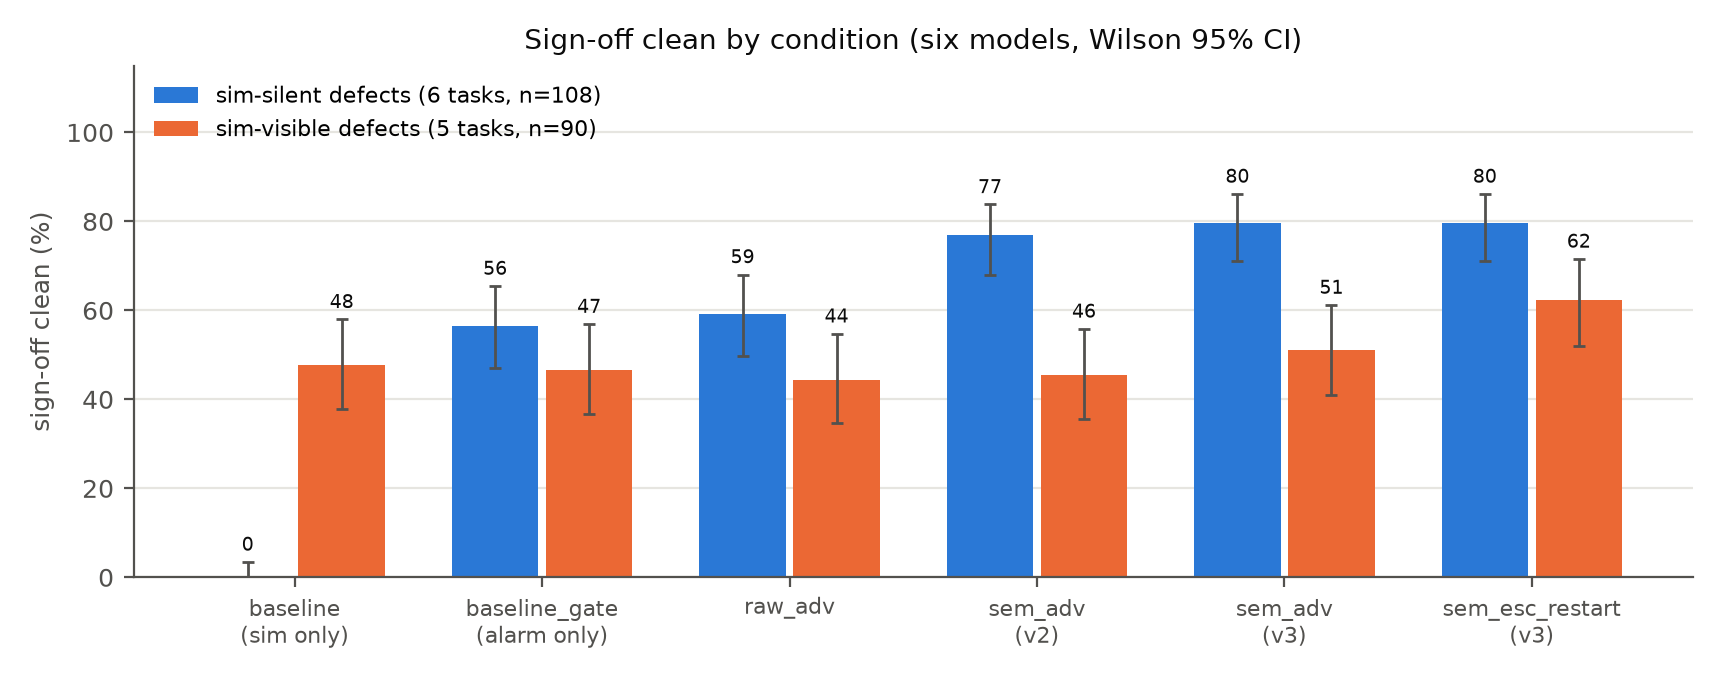
\includegraphics[width=\linewidth]{fig_p3_v2_clean_by_condition.png}
\caption{Sign-off clean by condition, split by whether the defect is visible to
simulation (six models, Wilson $95\%$ CI).}
\label{fig:cond}
\end{figure}

\subsection{What the model is told decides the repair}
\label{sec:res-gate}

The control arm answers the question the escalation design left open: is
escalation's gain the alarm or the detail? Told only that sign-off failed,
\texttt{baseline\_gate} reaches $52\%$ sign-off clean, level with raw tool text
($53\%$) and far below interpreted feedback ($63\%$ v2, $67\%$ v3) and
escalation ($72\%$). Table~\ref{tab:primary} gives the four pre-registered
contrasts. Contrasts~1 and~2 both exclude zero with the alarm lower: the
pre-registered reading is R1, \emph{the detail in the feedback adds value
beyond the verdict}. Table~\ref{tab:sens} shows the reading is the same under
the pre-declared processor-level sensitivity (Address\_select signed off by its
loop testbench, Section~\ref{sec:res-oracle}) and under the as-run metric.

\begin{table}[htbp]
\centering
\caption{Pre-registered primary contrasts on sign-off clean, six models.
Points, cell-level bootstrap $95\%$ CI, sign-flip $p$ over (model, task)
cells, discordant runs A-only/B-only.}
\label{tab:primary}
\small
\begin{tabular}{@{}l l c c c@{}}
\toprule
\textbf{Contrast (A $-$ B)} & \textbf{Tasks} & \textbf{$\Delta$ [CI]} & \textbf{$p$} & \textbf{A/B only} \\
\midrule
1. sem\_esc\_restart $-$ baseline\_gate & all         & $\mathbf{+19.7}$ [$+11.1$, $+29.3$] & ${<}0.001$ & $42/3$ \\
                                        & sim-silent  & $+23.1$ [$+11.1$, $+37.0$] & $0.002$ & $27/2$ \\
                                        & sim-visible & $+15.6$ [$+4.4$, $+27.8$]  & $0.022$ & $15/1$ \\
2. sem\_adv (v3) $-$ baseline\_gate     & all         & $\mathbf{+14.6}$ [$+3.0$, $+26.3$] & $0.021$ & $43/14$ \\
                                        & sim-silent  & $+23.1$ [$+6.5$, $+39.8$]  & $0.014$ & $31/6$ \\
                                        & sim-visible & $+4.4$ [$-11.1$, $+20.0$]  & $0.688$ & $12/8$ \\
3. baseline\_gate $-$ raw\_adv          & all         & $-0.5$ [$-9.1$, $+8.1$]    & $1.000$ & $16/17$ \\
                                        & sim-silent  & $-2.8$ [$-13.0$, $+7.4$]   & $0.738$ & $6/9$ \\
                                        & sim-visible & $+2.2$ [$-11.1$, $+15.6$]  & $0.882$ & $10/8$ \\
4. baseline\_gate $-$ baseline          & sim-visible & $-1.1$ [$-4.4$, $+2.2$]    & $1.000$ & $2/3$ \\
\bottomrule
\end{tabular}
\end{table}

\begin{table}[htbp]
\centering
\caption{The primary contrasts (all tasks) under the pre-declared
processor-level sensitivity and under the as-run metric. Points with
cell-level CI.}
\label{tab:sens}
\small
\begin{tabular}{@{}l c c@{}}
\toprule
\textbf{Contrast} & \textbf{Processor-level view} & \textbf{As run (loop testbench)} \\
\midrule
1. sem\_esc\_restart $-$ baseline\_gate & $+24.2$ [$+14.6$, $+34.3$] & $+23.7$ [$+14.1$, $+33.8$] \\
2. sem\_adv (v3) $-$ baseline\_gate     & $+19.7$ [$+7.6$, $+32.3$]  & $+17.7$ [$+5.1$, $+30.3$] \\
3. baseline\_gate $-$ raw\_adv          & $-3.0$ [$-12.1$, $+6.1$]   & $-3.0$ [$-12.1$, $+6.1$] \\
4. baseline\_gate $-$ baseline (sim-visible) & $-2.2$ [$-7.8$, $+3.3$] & $-2.2$ [$-7.8$, $+3.3$] \\
\bottomrule
\end{tabular}
\end{table}

\textbf{Why the alarm is not enough.} The alarm plateaus: after the third call
it adds two points ($50$ to $52\%$), while escalation, which opens with the
same message, climbs from $56$ to $72\%$ once it hands over to v3
(Figure~\ref{fig:call}). The alarm alone breaks working logic: on the
sim-silent tasks, where every run starts from RTL that already simulates, $80$
of $108$ alarm-only runs still pass the loop testbench at the end, against $97$
for escalation. And where it failed, the interpreter had something to say
(Table~\ref{tab:wouldfire}): of the $95$ alarm-only runs that are not sign-off
clean, v3 would have fired on the RTL the alarm was given on in all $95$, and
on the returned RTL in $38$. These are logged, never fed back, so they measure
availability, not effect.

\begin{table}[htbp]
\centering
\caption{\texttt{baseline\_gate}, six models: where the bare verdict was not
enough. \texttt{would\_fire}: v3 fires on at least one RTL the alarm was given
on; \texttt{would\_fire\_final}: on the returned RTL.}
\label{tab:wouldfire}
\small
\begin{tabular}{@{}l c c c c c@{}}
\toprule
\textbf{Task} & \textbf{Runs} & \textbf{Not sign-off} & \textbf{with}           & \textbf{with}                  & \textbf{Clean with} \\
              &               & \textbf{clean}        & \textbf{would\_fire}    & \textbf{would\_fire\_final}    & \textbf{would\_fire} \\
\midrule
Address\_select   & $18$ & $18$ & $18$ & $10$ & $0$ \\
MuxPC             & $18$ & $3$  & $3$  & $0$  & $15$ \\
execute\_mux      & $18$ & $6$  & $6$  & $0$  & $12$ \\
mem\_wb\_mux      & $18$ & $9$  & $9$  & $3$  & $9$ \\
mux3              & $18$ & $6$  & $6$  & $0$  & $12$ \\
ni\_flit\_pack    & $18$ & $14$ & $14$ & $6$  & $4$ \\
noc\_xbar4        & $18$ & $9$  & $9$  & $0$  & $9$ \\
register\_1bit    & $18$ & $8$  & $8$  & $6$  & $10$ \\
register\_32bit   & $18$ & $4$  & $4$  & $0$  & $14$ \\
register\_4bit    & $18$ & $3$  & $3$  & $0$  & $15$ \\
riscv\_alu\_flags & $18$ & $15$ & $15$ & $13$ & $3$ \\
\midrule
all               & $198$ & $95$ & $95$ & $38$ & $103$ \\
\bottomrule
\end{tabular}
\end{table}

\textbf{By model.} The detail matters most on the smallest models
(Figure~\ref{fig:models}). Escalation minus the alarm is $+39.4$ points on
llama3.2:3b ($19/33$ against $6/33$) and $+33.3$ on gemma3:4b ($17/33$ against
$6/33$), Holm $p=0.006$ each; on the other four models it is $+12.1$
(deepseek-coder:6.7b), $+18.2$ (qwen2.5-coder:7b), $+9.1$ (llama3.1:8b) and
$+6.1$ (qwen2.5-coder:14b), none individually significant after Holm
correction. By task, escalation minus the alarm is positive on ten of eleven
tasks and zero on \texttt{noc\_xbar4}; no single task survives Holm correction
across eleven.

\begin{figure}[htbp]
\centering
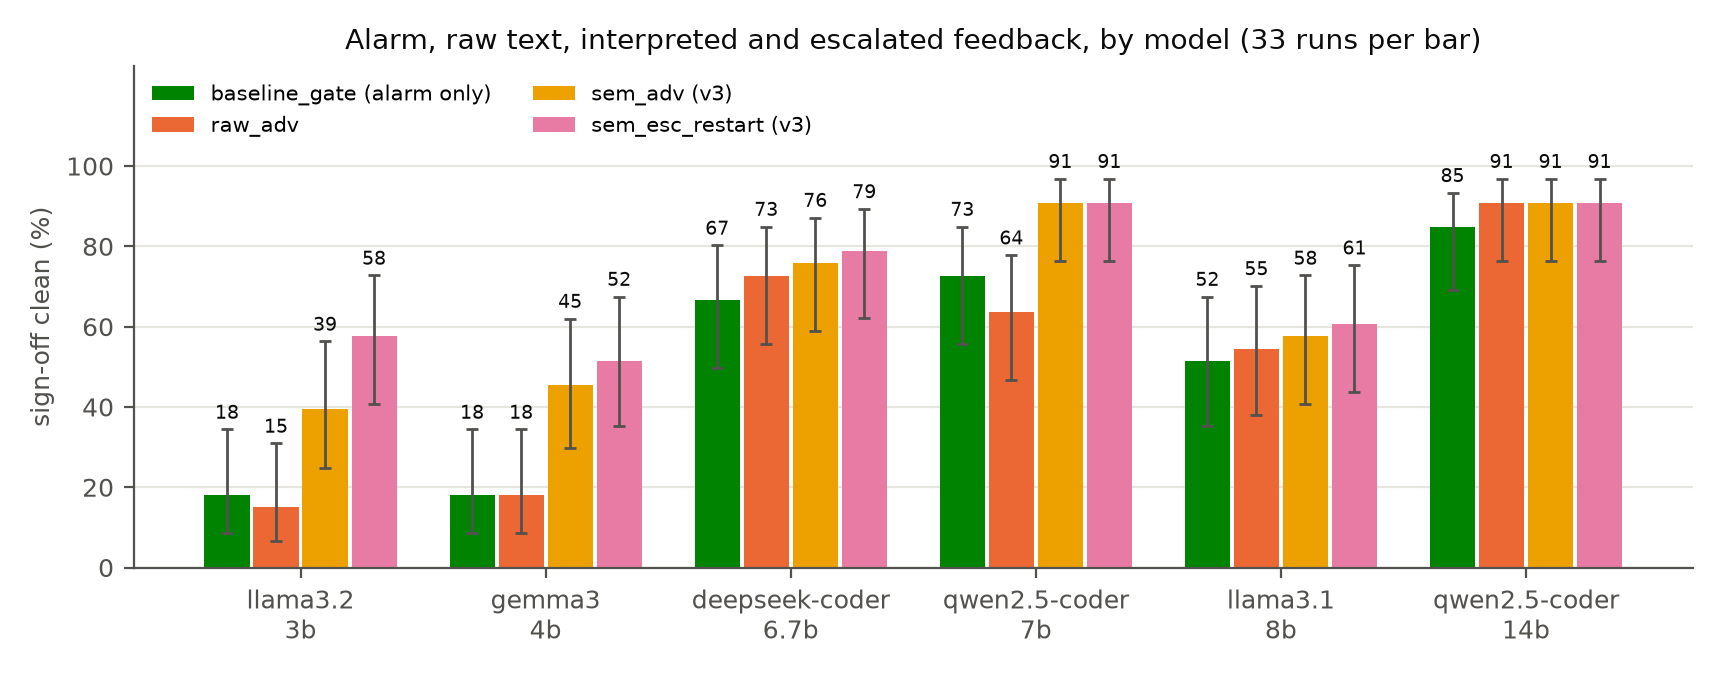
\includegraphics[width=\linewidth]{fig_p3_v2_by_model.png}
\caption{Sign-off clean per model under the alarm alone, raw tool text, v3
directives and escalation ($33$ runs per bar, Wilson $95\%$ CI).}
\label{fig:models}
\end{figure}

\subsection{Interpretation beats raw tool text, sooner and cheaper}
\label{sec:res-interp}

The cleanest test of interpretation is \texttt{sem\_adv} against
\texttt{raw\_adv}: the same raw text, the same budget, and directives as the
only difference. v3 reaches $132/198$ sign-off clean against $104/198$,
$+14.1$ points (cell-level CI $+3.5$ to $+24.7$, $p=0.014$, $40$ discordant
pairs in its favour against $12$; Table~\ref{tab:contrasts}). The production
interpreter, written before Phase~3 and never tuned on these designs, beats
raw text by $+10.1$ points (CI $+2.0$ to $+18.7$): the out-of-sample estimate
of what interpretation is worth. Both gains are carried by the sim-silent
tasks.

\begin{table}[htbp]
\centering
\caption{Re-stated contrasts on sign-off clean, six models. Points with
cell-level CI and sign-flip $p$; in the last column the as-run value.}
\label{tab:contrasts}
\small
\begin{tabular}{@{}l l c c c@{}}
\toprule
\textbf{A $-$ B} & \textbf{Tasks} & \textbf{$\Delta$ [CI]} & \textbf{$p$} & \textbf{As run} \\
\midrule
sem\_adv (v3) $-$ raw\_adv          & all        & $+14.1$ [$+3.5$, $+24.7$]  & $0.014$     & $+14.6$ \\
                                    & sim-silent & $+20.4$ [$+5.6$, $+35.2$]  & $0.016$     & $+16.7$ \\
                                    & sim-visible & $+6.7$ [$-7.8$, $+21.1$]  & $0.474$     & $+12.2$ \\
sem\_adv (v2) $-$ raw\_adv          & all        & $+10.1$ [$+2.0$, $+18.7$]  & $0.030$     & $+9.1$ \\
sem\_adv (v3) $-$ sem\_adv (v2)     & all        & $+4.0$ [$-4.0$, $+12.1$]   & $0.408$     & $+5.6$ \\
sem\_esc\_restart $-$ sem\_adv (v3) & all        & $+5.1$ [$-2.0$, $+12.6$]   & $0.255$     & $+6.1$ \\
sem\_esc\_restart $-$ raw\_adv      & all        & $+19.2$ [$+9.6$, $+28.8$]  & ${<}0.001$  & $+20.7$ \\
sem\_esc\_restart $-$ baseline      & sim-visible & $+14.4$ [$+3.3$, $+27.8$] & $0.048$     & $+23.3$ \\
\bottomrule
\end{tabular}
\end{table}

Interpretation is also the cheaper path (Table~\ref{tab:cost}): against raw
text, v3 uses about $23\%$ fewer model calls and tokens per run and spends
$5{,}066$ tokens per sign-off clean pass against $8{,}370$. It is faster:
$55\%$ of v3 runs are sign-off clean after the first call, against $41\%$ with
raw text, $40\%$ with the alarm and $15\%$ with simulation only
(Figure~\ref{fig:call}). Per model, v3 minus raw text is $+24.2$ points on
llama3.2:3b ($13/33$ against $5/33$), $+27.3$ on gemma3:4b ($15/33$ against
$6/33$), $+3.0$ on deepseek-coder:6.7b ($25/33$ against $24/33$), $+27.3$ on
qwen2.5-coder:7b ($30/33$ against $21/33$), $+3.0$ on llama3.1:8b ($19/33$
against $18/33$), and $0$ on qwen2.5-coder:14b ($30/33$ each).

\begin{table}[htbp]
\centering
\caption{Cost per condition, six models, $198$ runs each. Tool rounds: model
calls whose prompt carried tool feedback.}
\label{tab:cost}
\small
\begin{tabular}{@{}l r r r r r@{}}
\toprule
\textbf{Condition} & \textbf{Calls/} & \textbf{Tool rounds/} & \textbf{Tokens/} & \textbf{Tokens per} & \textbf{Clean by} \\
                   & \textbf{run}    & \textbf{run}          & \textbf{run}     & \textbf{sign-off clean} & \textbf{call 1} \\
\midrule
baseline               & $1.34$ & $0.00$ & $1{,}425$ & $6{,}562$ & $15\%$ \\
raw\_adv               & $3.27$ & $3.27$ & $4{,}396$ & $8{,}370$ & $41\%$ \\
sem\_adv (v2)          & $2.83$ & $2.83$ & $3{,}831$ & $6{,}117$ & $46\%$ \\
sem\_adv (v3)          & $2.51$ & $2.51$ & $3{,}377$ & $\mathbf{5{,}066}$ & $\mathbf{55\%}$ \\
sem\_esc\_restart (v3) & $2.99$ & $\mathbf{1.32}$ & $3{,}798$ & $5{,}295$ & $42\%$ \\
baseline\_gate         & $3.39$ & $0.00$ & $3{,}835$ & $7{,}372$ & $40\%$ \\
\bottomrule
\end{tabular}
\end{table}

\begin{figure}[htbp]
\centering
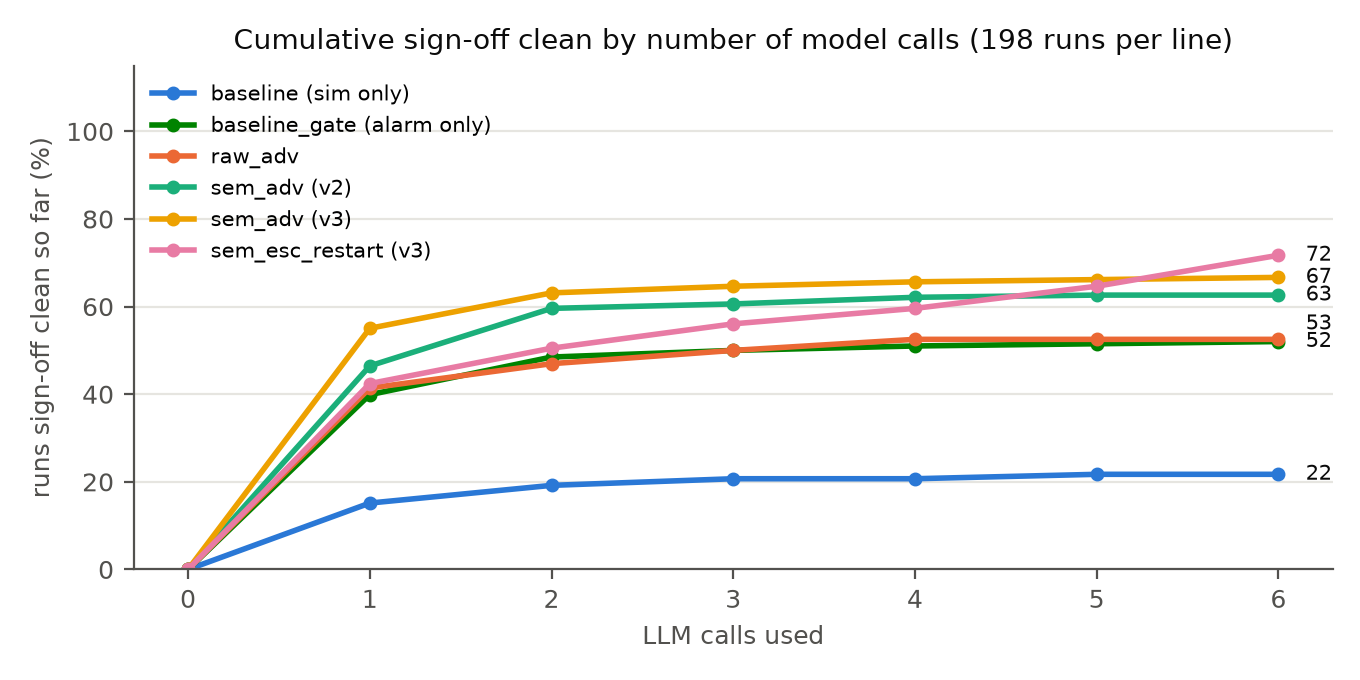
\includegraphics[width=0.85\linewidth]{fig_p3_v2_clean_by_call.png}
\caption{Share of runs sign-off clean after each number of model calls ($198$
runs per line). v3 front-loads its repairs; the alarm alone plateaus;
escalation, which opens with the same alarm, climbs to the highest final
rate.}
\label{fig:call}
\end{figure}

\subsection{Per task}
\label{sec:res-task}

Table~\ref{tab:pertask} gives every task. The latch multiplexers are where
interpretation is most decisive: simulation-only repair never touches them, and
\texttt{MuxPC} and \texttt{mux3} reach $18/18$ under both interpreters. Only
two tasks change between the oracles: \texttt{Address\_select}, where most
loop-clean repairs violate the specification, and \texttt{mem\_wb\_mux}
(Section~\ref{sec:res-oracle}). Three tasks stay at or below half under every
condition: \texttt{Address\_select} under the sign-off oracle, the multi-driven
crossbar (\texttt{noc\_xbar4}, $9$ to $10$ of $18$ everywhere) and the ALU
flags (\texttt{riscv\_alu\_flags}, at most $9/18$). They mark where the
vocabulary needs to go next.

\begin{table}[htbp]
\centering
\caption{Sign-off clean per task, $k/18$ ($6$ models $\times$ $3$
replicates); as-run value in brackets where it differs.}
\label{tab:pertask}
\small
\begin{tabular}{@{}l c c c c c c@{}}
\toprule
\textbf{Task} & \textbf{baseline} & \textbf{raw\_adv} & \textbf{v2} & \textbf{v3} & \textbf{esc (v3)} & \textbf{gate} \\
\midrule
\multicolumn{7}{@{}l}{\emph{Sim-silent}} \\
MuxPC             & $0$  & $17$ & $18$ & $18$ & $18$ & $15$ \\
execute\_mux      & $0$  & $10$ & $15$ & $15$ & $17$ & $12$ \\
mem\_wb\_mux      & $0$  & $9$ [$15$] & $11$ [$14$] & $11$ [$13$] & $11$ [$16$] & $9$ [$15$] \\
mux3              & $0$  & $12$ & $18$ & $18$ & $17$ & $12$ \\
register\_1bit    & $0$  & $10$ & $12$ & $15$ & $16$ & $10$ \\
riscv\_alu\_flags & $0$  & $6$  & $9$  & $9$  & $7$  & $3$ \\
\midrule
\multicolumn{7}{@{}l}{\emph{Sim-visible}} \\
Address\_select   & $0$ [$3$] & $1$ [$8$] & $1$ [$9$] & $2$ [$14$] & $4$ [$15$] & $0$ [$2$] \\
register\_32bit   & $15$ & $11$ & $12$ & $15$ & $16$ & $14$ \\
register\_4bit    & $14$ & $10$ & $11$ & $14$ & $17$ & $15$ \\
noc\_xbar4        & $10$ & $9$  & $10$ & $9$  & $9$  & $9$ \\
ni\_flit\_pack    & $4$  & $9$  & $7$  & $6$  & $10$ & $4$ \\
\bottomrule
\end{tabular}
\end{table}

\subsection{The v3 upgrade: the right directive on every task}
\label{sec:res-v3}

Coverage is where the upgrade is unambiguous (Table~\ref{tab:upgrade}). On
\texttt{register\_1bit} and \texttt{ni\_flit\_pack} the production
interpreter produced no directive on the defective input in any of $18$ runs;
v3 fires the intended class in all $18$. On the two latching registers v2
directed the model to gate on the clock; v3 names the missing clock edge. On
\texttt{Address\_select} v2 added a misleading ``gate the output on the
instruction bus'' directive, which v3 suppresses. On the four tasks singled out
before the runs (the two silent and the two misleading ones, none of which has
a differing sign-off testbench), sign-off clean passes rise from $42/72$ to
$50/72$ ($+11.1$ points, cell CI $-9.7$ to $+31.9$); on \texttt{register\_1bit}
the interpreter-credited wins rise from $3/18$ to $15/18$. The pass-rate gain
is in the favourable direction at this $N$, and because v3 was written from
these designs' logs, it remains in-sample until tested on held-out defects.

\begin{table}[htbp]
\centering
\caption{Where production v2 was silent or misleading. Fired: runs in which
the interpreter produced a directive on the defective input ($/18$).
Clean: sign-off clean ($/18$), as-run in brackets where it differs.}
\label{tab:upgrade}
\small
\begin{tabularx}{\linewidth}{@{} l X c c c c @{}}
\toprule
\textbf{Task} & \textbf{v2 on the input} & \textbf{v2 fired} & \textbf{v3 fired} & \textbf{v2 clean} & \textbf{v3 clean} \\
\midrule
register\_1bit  & silent (abort unhandled)          & $0$  & $18$ & $12$ & $15$ \\
ni\_flit\_pack  & silent (expression truncation)    & $0$  & $18$ & $7$  & $6$ \\
register\_32bit & gate on the clock (misleading)    & $18$ & $18$ & $12$ & $15$ \\
register\_4bit  & gate on the clock (misleading)    & $18$ & $18$ & $11$ & $14$ \\
Address\_select & extra gating directive on a bus   & $18$ & $18$ & $1$ [$9$] & $2$ [$14$] \\
\bottomrule
\end{tabularx}
\end{table}

\subsection{Escalation: highest clean rate, fewest tool rounds}
\label{sec:res-esc}

Escalation reaches the highest sign-off clean rate ($142/198$, $72\%$) and
keeps baseline's $85\%$ loop pass rate, with $1.32$ tool-feedback rounds per
run against $2.51$ for always-on v3 ($47.5\%$ fewer). On the sim-visible
tasks, where simulation-only repair does run the model, escalation beats it by
$+14.4$ points ($56/90$ against $43/90$, cell CI $+3.3$ to $+27.8$, $p=0.048$;
$+23.3$ as run, the difference being \texttt{Address\_select}). There,
deepseek-coder:6.7b reaches $13/15$ and qwen2.5-coder:7b $12/15$ against
baseline's $9/15$ each, and escalation protects the smallest model:
llama3.2:3b is at $7/15$ with simulation only, $1/15$ with raw text every
round, and $8/15$ with escalation. $109$ runs never needed to escalate ($100$
of them ended sign-off clean); the $89$ that did ended $42$ sign-off clean.

\subsection{Repaired leaves restore the real designs}
\label{sec:res-compose}

Each (model, replicate) set of final leaves was spliced back into the real
designs and re-synthesised (Table~\ref{tab:compose},
Figure~\ref{fig:compose}). Simulation-only repair never yields a synthesisable
design ($0/18$ in each), because it never touches the sim-silent register
that aborts synthesis. v3 restores top-level synthesis in $16/18$ groups for
each design, escalation in $18/18$ for both meshes, and the alarm alone in
$11/18$ for each, of which only $1$ MPSoC group reaches the golden bound. In
the $990$ runs, leaf-level \texttt{clean\_pass} was sufficient for composition
in every case: whenever all composed leaves were clean, the design reached the
golden bound of Table~\ref{tab:prop} ($32/32$ for each mesh, $27/27$ for the
MPSoC). For qwen2.5-coder:32b every tool condition composes $3/3$ at the bound
in all three designs, and baseline $0/3$.

\begin{table}[htbp]
\centering
\caption{Top-level synthesis pass after splicing in each condition's repaired
leaves ($18$ model $\times$ replicate groups per cell, six models), and in
brackets the groups that also reach the golden latch bound. Synthesis only.}
\label{tab:compose}
\small
\begin{tabular}{@{}l c c c c c c@{}}
\toprule
\textbf{Design} & \textbf{baseline} & \textbf{raw\_adv} & \textbf{v2} & \textbf{v3} & \textbf{esc (v3)} & \textbf{gate} \\
\midrule
$2{\times}2$ mesh & $0$ ($0$) & $15$ ($10$) & $13$ ($11$) & $16$ ($15$) & $\mathbf{18}$ ($\mathbf{16}$) & $11$ ($8$) \\
$3{\times}3$ mesh & $0$ ($0$) & $15$ ($10$) & $13$ ($11$) & $16$ ($15$) & $\mathbf{18}$ ($\mathbf{16}$) & $11$ ($8$) \\
MPSoC top         & $0$ ($0$) & $13$ ($8$)  & $12$ ($8$)  & $\mathbf{16}$ ($\mathbf{14}$) & $15$ ($13$) & $11$ ($1$) \\
\bottomrule
\end{tabular}
\end{table}

\begin{figure}[htbp]
\centering
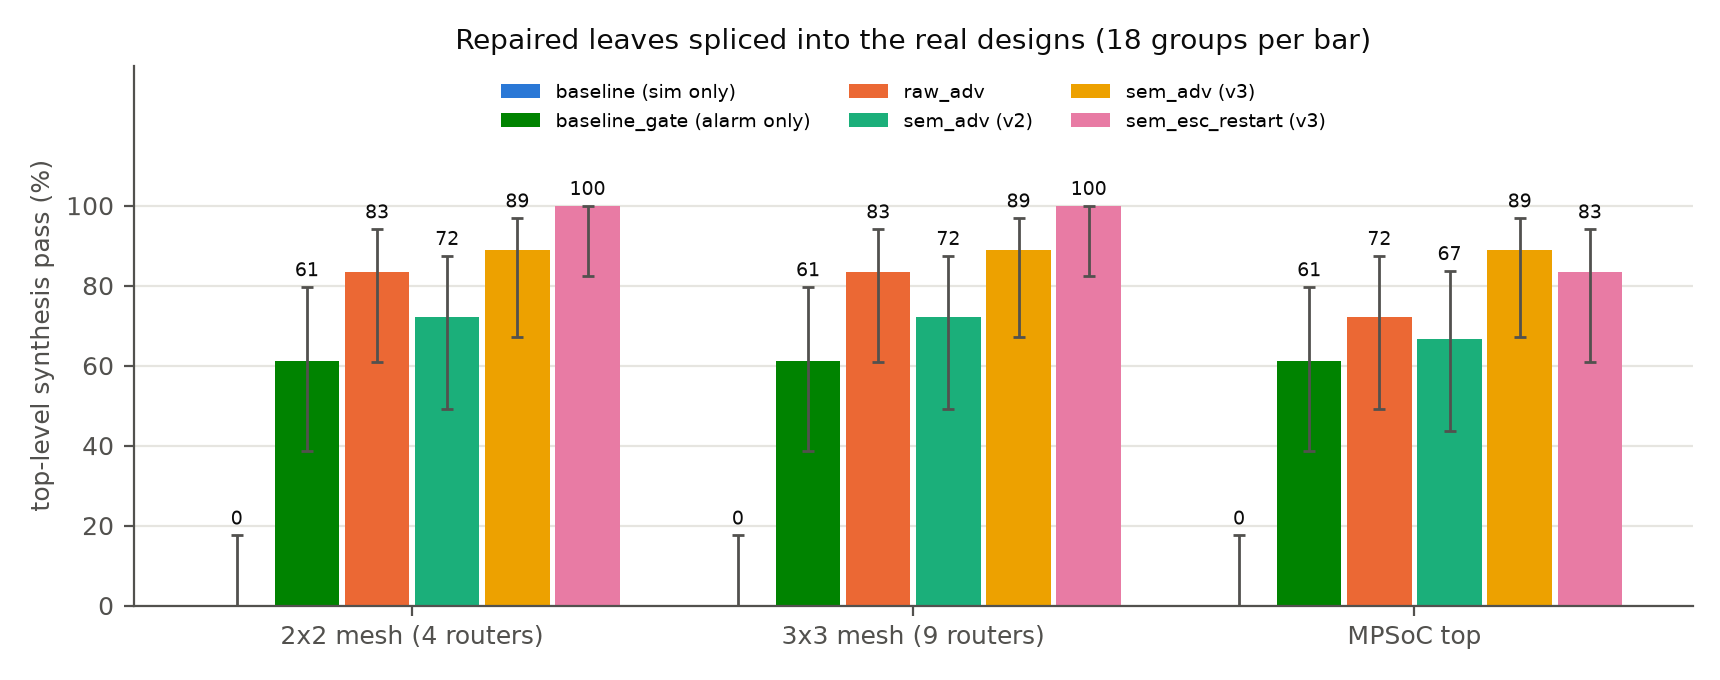
\includegraphics[width=\linewidth]{fig_p3_v2_composition.png}
\caption{Top-level synthesis pass of the two meshes and the MPSoC after
splicing in repaired leaves, by condition (Wilson $95\%$ CI).}
\label{fig:compose}
\end{figure}

\subsection{Oracle integrity, and a limitation of structural advice}
\label{sec:res-oracle}

Every clean repair was checked against the golden fix with Yosys
(\texttt{equiv\_make}, \texttt{equiv\_simple -seq 5}, \texttt{equiv\_induct}),
and its constant-driven output bits were counted; as a check of the flow, each
golden fix is shown equivalent to itself. Where a candidate was not proven equivalent, the
check was repeated with inputs the specification declares illegal mapped to a
legal value (select code $2'b11$ on \texttt{MuxPC} and \texttt{mux3}, a
non-one-hot grant on \texttt{noc\_xbar4}). No clean repair ties an output bit
to a constant beyond the golden fix. Table~\ref{tab:audit} gives the audit of
the sim-visible tasks and \texttt{mem\_wb\_mux}; on \texttt{MuxPC},
\texttt{execute\_mux}, \texttt{mux3}, \texttt{register\_1bit} and
\texttt{riscv\_alu\_flags} every clean repair is equivalent, or equivalent on
legal inputs.

\begin{table}[htbp]
\centering
\caption{Equivalence audit of the clean runs (all conditions of the $990$
runs). Class (i): the repair differs from the golden fix on behaviour the
specification defines, and the loop testbench does not check it.}
\label{tab:audit}
\small
\begin{tabular}{@{}l c c c c@{}}
\toprule
\textbf{Task} & \textbf{Clean runs} & \textbf{Equivalent} & \textbf{Equivalent on legal inputs} & \textbf{Class (i)} \\
\midrule
Address\_select  & $49$ & $8$  & $0$  & $41$ \\
ni\_flit\_pack   & $36$ & $36$ & $0$  & $0$ \\
noc\_xbar4       & $47$ & $0$  & $47$ & $0$ \\
register\_32bit  & $69$ & $69$ & $0$  & $0$ \\
register\_4bit   & $66$ & $66$ & $0$  & $0$ \\
mem\_wb\_mux     & $58$ & $42$ & $0$  & $16$ \\
\bottomrule
\end{tabular}
\end{table}

In \texttt{mem\_wb\_mux} the conference paper's motivating case appears in
real RTL: a latch holds a stale store operand in exactly the cases the loop
testbench never drives (\texttt{ex\_mem\_memwrite} $=0$, and forwarding code
\texttt{2'b11}), and $16$ loop-clean repairs drive a value other than the
specified one there. In \texttt{Address\_select} the specification defines
\texttt{J\_addr} $= X + \texttt{PC}$ on every input, the loop testbench checks
it only on a non-flushed jump, and $41$ loop-clean repairs set \texttt{J\_addr}
to $0$ elsewhere: latch-free and synthesisable, yet in
violation of the specification. For each gap the sign-off testbench passes the
golden fix, fails every class-(i) repair, still passes every other clean
repair, and fails a golden mutant that differs only in the unchecked cases.

The production latch directive, which v3 passes on for \texttt{Address\_select},
suggests ``one unconditional assignment at the top of the block'' of the form
\texttt{J\_addr = <safe value>}. Table~\ref{tab:advice} counts, per condition,
the runs that are loop clean but fail sign-off (gap runs) and how many received
that advice (pre-declared, exploratory). Simulation only, raw text and the
alarm produce gap runs without it, so this is a count, not a causal claim. On
\texttt{mem\_wb\_mux} the same advice also reached every v2 and v3 run that
ended sign-off clean ($11/11$ each). At the processor level the
\texttt{Address\_select} violation is invisible, since MuxPC reads
\texttt{J\_addr} only when \texttt{PCsrc} $= 01$; the pre-declared sensitivity
that signs \texttt{Address\_select} off with its loop testbench gives the same
pre-registered reading (Table~\ref{tab:sens}).

\begin{table}[htbp]
\centering
\caption{Gap runs (loop clean, failing sign-off), six models, and how many
received the production latch text (``\texttt{<safe value>}'' at the top of
the block) in any feedback round.}
\label{tab:advice}
\small
\begin{tabular}{@{}l c c c c c c@{}}
\toprule
 & \textbf{baseline} & \textbf{raw\_adv} & \textbf{v2} & \textbf{v3} & \textbf{esc (v3)} & \textbf{gate} \\
\midrule
Address\_select: gap runs       & $3$ & $7$ & $8$ & $12$ & $11$ & $2$ \\
\quad with the advice           & $0$ & $0$ & $8$ & $12$ & $11$ & $0$ \\
mem\_wb\_mux: gap runs          & $0$ & $6$ & $3$ & $2$  & $5$  & $6$ \\
\quad with the advice           & $0$ & $0$ & $3$ & $2$  & $0$  & $0$ \\
\bottomrule
\end{tabular}
\end{table}

\subsection{Up the ladder}
\label{sec:res-ladder}

Table~\ref{tab:ladder} adds qwen2.5-coder:32b (pre-registered) and the two API
models (descriptive), one model each at $N{=}3$. At this size any tool feedback
repairs every sim-silent defect ($18/18$ under every tool condition, $16$ or
$18$ under the alarm alone); every miss outside baseline is the
\texttt{Address\_select} gap, apart from two alarm-only runs on
\texttt{riscv\_alu\_flags} for qwen2.5-coder:32b and for gpt-4.1-mini. So
interpretation's edge over raw text and over the alarm vanishes at the top of
the ladder, while simulation-only repair still signs off all $18$ sim-silent
runs as defective for every model: the guard is needed at every size, and the
translation matters most for small models.

\begin{table}[htbp]
\centering
\caption{Ladder rows ($33$ runs per cell, $N{=}3$; not pooled with
Table~\ref{tab:pooled}). Sign-off clean of $33$ with sim-silent (of $18$) and
sim-visible (of $15$) counts, and tokens per run.}
\label{tab:ladder}
\small
\begin{tabular}{@{}l cr cr cr@{}}
\toprule
 & \multicolumn{2}{c}{\textbf{qwen2.5-coder:32b}} & \multicolumn{2}{c}{\textbf{gpt-4.1-mini}} & \multicolumn{2}{c}{\textbf{claude-haiku-4.5}} \\
\cmidrule(lr){2-3}\cmidrule(lr){4-5}\cmidrule(l){6-7}
\textbf{Condition} & \textbf{clean} & \textbf{tokens} & \textbf{clean} & \textbf{tokens} & \textbf{clean} & \textbf{tokens} \\
\midrule
baseline               & $12$ ($0$/$12$)  & $663$     & $12$ ($0$/$12$)  & $440$     & $12$ ($0$/$12$)  & $517$ \\
baseline\_gate         & $28$ ($16$/$12$) & $1{,}824$ & $28$ ($16$/$12$) & $1{,}529$ & $30$ ($18$/$12$) & $1{,}099$ \\
raw\_adv               & $30$ ($18$/$12$) & $1{,}492$ & $30$ ($18$/$12$) & $1{,}164$ & $30$ ($18$/$12$) & $1{,}334$ \\
sem\_adv (v2)          & $30$ ($18$/$12$) & $1{,}655$ & $30$ ($18$/$12$) & $1{,}255$ & $30$ ($18$/$12$) & $1{,}517$ \\
sem\_adv (v3)          & $30$ ($18$/$12$) & $1{,}660$ & $30$ ($18$/$12$) & $1{,}257$ & $30$ ($18$/$12$) & $1{,}524$ \\
sem\_esc\_restart (v3) & $30$ ($18$/$12$) & $1{,}850$ & $30$ ($18$/$12$) & $1{,}404$ & $30$ ($18$/$12$) & $1{,}101$ \\
\bottomrule
\end{tabular}
\end{table}

In the seven-model sensitivity pool (the six models plus qwen2.5-coder:32b),
every contrast keeps its sign: escalation minus the alarm is $+17.7$ points
(CI $+10.4$ to $+25.6$) and v3 minus the alarm $+13.4$ (CI $+3.5$ to $+23.8$).

% ============================================================================
\section{What Phase 3 Establishes, and What Comes Next}
\label{sec:summary}

On real multiprocessor RTL the question is not whether a module simulates but
whether the design can be signed off. There, a simulation-only loop is
structurally blind at every model size tested: it signed off every
simulation-silent defect in this study. The synthesis and lint layer makes
those defects visible, and what the model is then told decides the repair: the
alarm that sign-off failed is worth about as much as raw tool text, while
interpretation adds $14.6$ points and escalation $19.7$, most on the smallest
models, sooner and more cheaply than raw text. Leaf repairs compose: a handful
of repaired definitions restores synthesis of networks with $4$ and $9$
routers and of the processor top. The interpreter can keep up with new
designs: real logs exposed missing vocabulary, and an additive,
regression-gated layer closed it without disturbing earlier results.

Limits: the v3 rules are in-sample; the sign-off oracle is post hoc for the
first $990$ runs (pre-registered for the rest, with the as-run metric reported
beside it); the control arm ran on a different inference backend, with no
detectable effect; the $32$B and API rows are one model each at $N{=}3$, at the
task set's ceiling; composition is checked by synthesis only; and replicates
are correlated, so general claims rest on the cell-level bootstrap.

Next:
\begin{enumerate}[leftmargin=1.2em, itemsep=0.1em]
\item \textbf{Held-out defects} for the v3 rules, which were written from
these designs' logs.
\item \textbf{A specification-valued default.} A latch directive that tells the
model to default each signal to the value the specification defines, rather
than to a constant, addresses the \texttt{Address\_select} gap runs.
\item \textbf{Keeping the best candidate.} Some runs pass simulation at some
point (the defective input included) and lose it later ($23$ of $198$ under
v3, $11$ under escalation in the $990$ runs); returning the best candidate so
far would recover them.
\item \textbf{More replicates} on the tasks that stayed flat
(\texttt{noc\_xbar4}, \texttt{riscv\_alu\_flags}), and integration-level
feedback for defects that only exist once modules are connected (a one-bit
program-counter port driven with $32$ bits, a FIFO instantiated positionally
with a missing port).
\end{enumerate}

\end{document}
